% English documentation/comments as requested.
% Build: xelatex cv-devops.tex  (or lualatex)

\documentclass[10pt,a4paper]{article}

\usepackage[T1]{fontenc}
\usepackage[utf8]{inputenc}
\usepackage{lmodern}
\usepackage[a4paper,margin=1.5cm]{geometry}

\usepackage{xcolor}
\usepackage{hyperref}
\usepackage{graphicx}
\usepackage{enumitem}
\usepackage{titlesec}
\usepackage{fontspec}

\definecolor{primary}{HTML}{1F4E79}

\hypersetup{colorlinks=true, linkcolor=primary, urlcolor=primary}

\titleformat{\section}{\large\bfseries\color{primary}}{}{0pt}{}

\setlist[itemize]{noitemsep, topsep=2pt, leftmargin=*, label=\textcolor{primary}{\textbullet}}

\newcommand{\resumeSection}[1]{\section*{#1}\vspace{-2mm}}
\newcommand{\smallGap}{\vspace{-1mm}}

\IfFontExistsTF{Fira Sans}{\setmainfont{Fira Sans}}{\setmainfont{DejaVu Sans}}

\begin{document}

\noindent
\begin{minipage}[t]{0.71\textwidth}
  {\LARGE\bfseries Pierre Courteille}\smallGap\\
  {\small He/Him}\\[2pt]
  {\normalsize\color{primary}\textbf{Cloud Architect (Freelance) $\mid$ AWS $\mid$ DevOps $\mid$ CDK $\mid$ Terraform}}\\
  {\small SaaS $\cdot$ Multi-Account (Organizations) $\cdot$ 4x AWS Certified}\\[4pt]
  {\normalsize
    (+33) 6 08 04 22 44 \hspace{6pt} $\vert$ \hspace{6pt}
    \href{mailto:pierre.courteille@gmail.com}{pierre.courteille@gmail.com}\\[2pt]
    \href{https://www.linkedin.com/in/pierre-courteille-b7432b186/}{LinkedIn} \hspace{6pt} $\vert$ \hspace{6pt}
    Geneva, Switzerland
  }
\end{minipage}
\hfill
\begin{minipage}[t]{0.22\textwidth}
  \raggedleft
  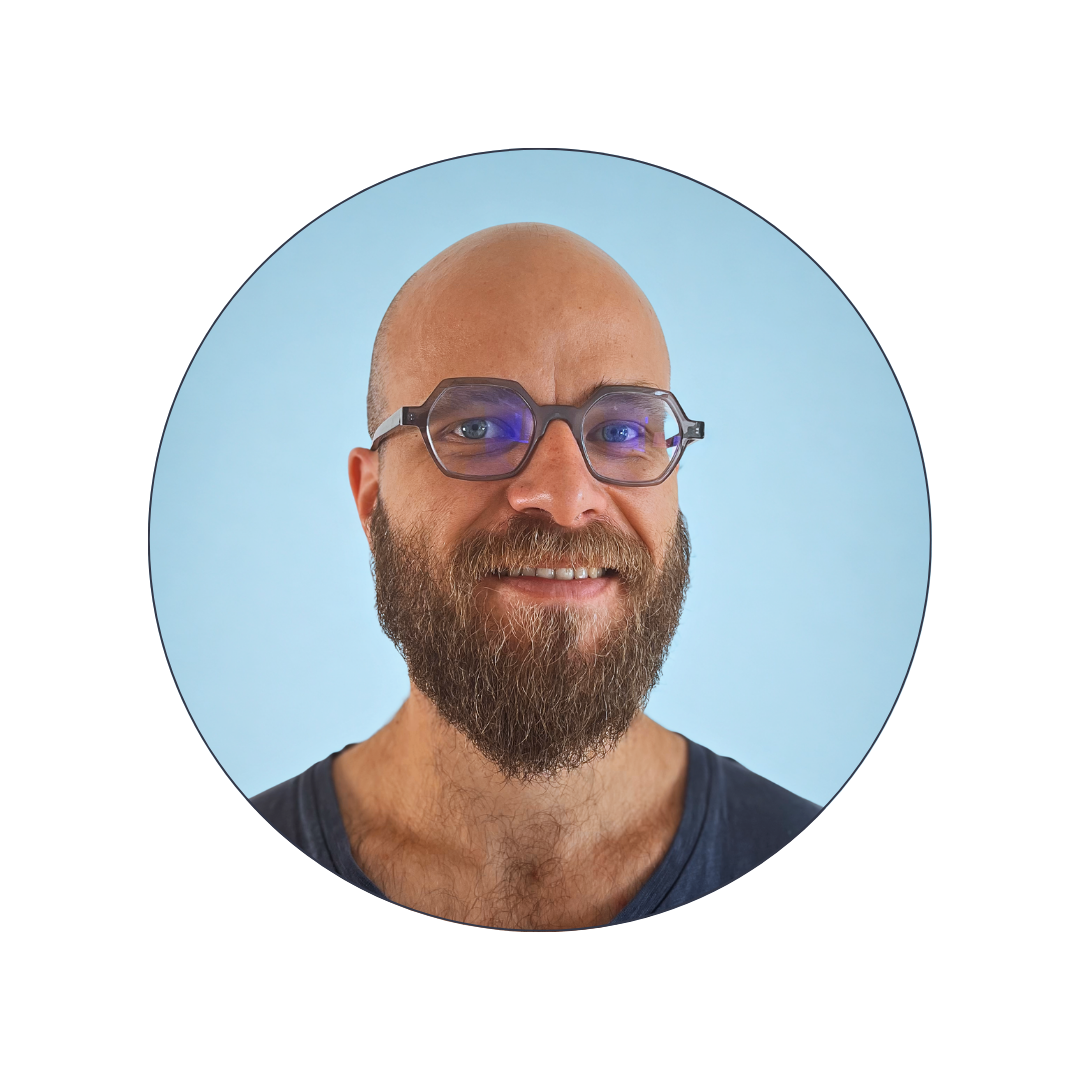
\includegraphics[width=1.75cm,height=1.75cm,keepaspectratio]{photo/face_circle.png}
\end{minipage}

\vspace{2mm}

\resumeSection{Profile}
\begin{itemize}
  \item Cloud \& DevOps on AWS (4x certified): architecture, security, automation; design, migrate, optimize with focus on scalability and performance.
  \item CI/CD; IaC (CDK, CloudFormation); resilient platforms. AWS: EKS, EC2, ECS, Lambda, RDS, VPC, CDK, SAM, IAM, etc.
  \item 8+ years; 20+ clients. Priorities: security, performance, scalability, robustness.
  \item Strong interest in complex problems mixing cloud and math/optimization.
\end{itemize}

\resumeSection{Experience}
\textbf{Cloud Engineer (contract) - Qim info / IEC} \hfill \emph{Oct 2025 -- Present}\\
\textit{Geneva, Switzerland} --- Multi-account AWS for IEC; SaaS silo (1 tenant = 1 account, Organizations); CDK, ECS Fargate; OAM, Grafana, WAF, Athena; Python.
\smallGap
\textbf{Cloud Engineer (freelance) - Premaccess} \hfill \emph{Jun 2019 -- Sep 2025}\\
\textit{Paris, France} --- Client migrations \& scale: ECS/EKS, Lambda, RDS, DynamoDB; VPC, IAM IC, SCPs, KMS; CI/CD; FinOps; BAM (Python/Boto3); C\# (+40\% / --30\%); SAM; L2/L3.
\smallGap
\textbf{CEO - CUBITO} \hfill \emph{Apr 2023 -- Aug 2025} \quad \textit{Ern\'ee, France}
\smallGap
\textbf{.NET Instructor \& SWE (freelance) - ISIKA} \hfill \emph{Mar 2020 -- Apr 2023}\\
\textit{Paris, France} --- C\#, OOP, WinForms; LINQ, EF, MySQL; project coaching.
\smallGap
\textbf{Software QA Manager - Bassetti} \hfill \emph{Feb 2016 -- May 2018}\\
\textit{Kolkata, India} --- 25+ QA engineers; API automation ($>$10k/h); DevOps practices; C\#, Selenium, Jenkins.
\smallGap
\textbf{Optimization Engineer - Kronos (Ad Opt)} \hfill \emph{Jan 2015 -- Jan 2016}\\
\textit{Montreal, Canada} --- Airline crew planning; column generation, shortest path; GERAD; C/C++, Linux, Git.

\resumeSection{Certifications (through Jul 2028)}
\begin{itemize}
  \item AWS Developer - Associate; DevOps Engineer - Professional; Solutions Architect - Associate (Jul 2025)
  \item AWS Cloud Practitioner (Jun 2025)
\end{itemize}

\resumeSection{Education}
\begin{itemize}
  \item Master's (MOCA) -- Universit\'e de Montpellier (2012--2015)
  \item Bachelor's, Math \& CS -- Universit\'e de Nantes (2009--2012)
\end{itemize}

\end{document}
